\documentclass[conference]{IEEEtran}
%IEEEoverridecommandlockouts
% The preceding line is only needed to identify funding in the first footnote. If that is unneeded, please comment it out.
\usepackage{cite}
\usepackage{amsmath,amssymb,amsfonts}
\usepackage{algorithmic}
\usepackage{graphicx}
\usepackage{textcomp}
\usepackage{xcolor}
\usepackage{pgfplots}
\usepackage{listings}
\usepackage{multicol}
\usepackage{graphicx}
\usepackage{amsmath}
\def\BibTeX{{\rm B\kern-.05em{\sc i\kern-.025em b}\kern-.08em
    T\kern-.1667em\lower.7ex\hbox{E}\kern-.125emX}}
\begin{document}

\title{Optimal Assignment Problem}

\author{\IEEEauthorblockN{Lekhana Mitta}
\IEEEauthorblockA{\text{IIT2019204} \\
}
\and
\IEEEauthorblockN{Sanskar Patro}
\IEEEauthorblockA{\text{IIT2019205} \\
}
\and
\IEEEauthorblockN{Aamin Chaudhari}
\IEEEauthorblockA{\text{IIT2019206} \\
}

}

\maketitle

\begin{abstract}
Suppose there are n jobs to be performed and n persons are available for doing these jobs. Assume that each person can do each job at a term, though with varying degree of efficiency.
The problem is to find an assignment so that the total cost of performing all jobs is minimum, problem of this kind are known as assignment problem.
\end{abstract}

\begin{IEEEkeywords}
combinatorics, matrices, minimisation, cost
\end{IEEEkeywords}

\section{Introduction}
This document describes the procedure followed to find the optimal assignment solution.

\section{Algorithm Design}

\subsection{Combinatorial Optimization}

Combinatorial optimization is a topic that consists of finding an optimal object from a finite set of objects. It has important applications in several fields, including artificial intelligence, machine learning, auction theory, software engineering, etc. The Hungarian method is a combinatorial optimization algorithm that solves the assignment problem in polynomial time

\subsection{Working}

This algorithm works on the principle of reducing the given cost matrix to a matrix of opportunity costs.

Opportunity cost shows the relative penalties associated with assigning people to a job as opposed to making the best or least cost assignment. If we can reduce the cost matrix to the extent of having at least one zero in each row and column, it will be possible to make optimal assignment.


\section{Algorithmic Analysis}


\emph{Steps in the Hungarian Method:}\\
To find the minimum cost arrangement,
\begin{enumerate}
% Input phase:\\
\item The user inputs the number of test cases and it is stored in a variable t.
\item Next, the user has to input the number of jobs and persons. This is stored in a variable n.
\item For every test case we use random number generation function to fill an n*n cost matrix whose cells contains the efficiency of each person at each job.
% \\Processing the matrix:\\
\item Find the element with minimum cost in each row of the cost matrix. Then subtract all values in that row with this minimum value.
% \\Looking for assignments:\\
\item Find the element with minimum cost in each column of the cost matrix. Then subtract all values in that column with this minimum value.
\item Examine rows successively until a row with exactly one unmarked zero is obtained. Make an assignment single zero by making a square around it.
\item For each zero value that becomes assigned, eliminate (Strike off) all other zeros in the same row and/ or column.
\item Repeat steps 6 and 7 for each successive column also with exactly single zero value all that has not been assigned.
\item If some row/column has two or more unmarked zeros and one cannot be chosen by inspection, then choose the assigned zero cell arbitrarily.
\item Continue this process until all zeros in row column are either assigned or struck off.
\item Now, if the number of assigned cells is equal to the number of rows/columns then it is the optimal solution. 
\item The total cost associated with this solution is obtained by adding original cost figures in the occupied cells.
\item If the number of assigned cells is not equal to the number of rows/columns, further processing is required.

\end{enumerate}


\section{Pseudo Code}
\lstset { %
    language=C++,
    backgroundcolor=\color{black!6},
    basicstyle=\footnotesize,
}
\begin{lstlisting}


Main Function : 

int size <- rand() 
func1(int m)

func1 Function :
int**matrix .
for i <- 0 to size 
  for j <- 0 to size
	  matrix[i][j] <- rand()%20 + 1
func2(int**matrix,int m)
	
func2 function :
int** spare_matrix <- matrix
func3(matrix,size)
func4(matrix,size)			
func6(matrix,size)			
func3(matrix ,size)
point** final_matrix 
    <- func8(matrix, size)
if(func14(final_matrix, size) ! <- 0)
	func15(final_matrix, size);
    func16(final_matrix, size);
	answer <- 
	func17(spare_matrix, final_matrix, size);
	print answer
	
func3 function : 
for i <- 0 to size
	for j <- 0 to size.
		print matrix 

func4 function : 
for i <- 0 to size
	int min <- 
	    func5(matrix[i], size);
	for l <- 0 to size
		matrix[i][l] <- 
		    matrix[i][l] - min

func5 function : 
min <- matrix[0][x]
for i <- 0 to size	
	if matrix[i][x] < min
	min <- matrix[i][x]
	return min
	
func6 function :
for i <- 0 to size
	int min <-
	func7(int **matrix,
	    int column_index,int size)
	for l <- 0 to size
		matrix[i][l] <- 
		    matrix[i][l] - min

func7 function :
min <- matrix[x][0]
for i <- 0 to size	
	if matrix[x][i] < min
		min <- matrix[x][i]
return min
	
func8 function : 
point** new_matrix <- copy(matrix)
for i <- 0 to size	
	func9(new_matrix, size, i)
return matrix
	
	
func9 function :
bool flag <- false
for l <- 0 to size
	new_matrix[l][i].data <- 0
		int row_index <- func10
		    (new_matrix, size, l)
		if row_index <- -1
			flag <- true
			new_matrix[l][i].used 
			    <- 1
			break
	
if flag !<- 1
	for l <- 0 to size
		if new_matrix[l][i].data
		    <- 0
			int column_index <- 
			func10(new_matrix, size, l)
			if 
			func11
			(new_matrix, size,
			    column_index, i) !<- 0
				new_matrix[l][i].used 
				<- 1
				new_matrix[l]
				[column_index].used 
				<- 0
				break
			else
				new_matrix[l][i].used 
				<- 2
	
func13(new_matrix, size)


func10 function :
for i <- 0 to size
	if points[row_index][i].used <- 1 
	    & points[row_index][i].data <- 0
		return i;
return -1;
	
func11 function : 
if start_column == column	
	return false
int count = 0;
for i <- 0 to size
	if new_matrix[i][column].data<- 0
		count <- count + 1
		index <- 
		    func10(new_matrix, size, i)
			if index <- -1
			func12(new_matrix, size
			, column)
			new_matrix[i][column].used 
			<- 1
			return true

if count <- 1
	return false
for j <- 0 to size
	if new_matrix[j][column].data <- 0
		count <- count + 1
		index <- 
		    func10(new_matrix, size, l)
		if index <- -1
			func11(new_matrix, size, 
		     column_index, start_column)
			new_matrix[j][column].used
			    <- 1
			return true
return false
	
func12 function :
for l <- 0 to size	
	if matrix[l][column_index].data <- 0 
	    && matrix[l][column_index] <- 1
		matrix[l][column_index].used <- 0
		break;

func13 function :
temp <- temp + 1
print temp
for i <- 0 to size 
	for l <- 0 to size
		print matrix[i][l].data 
		print matrix[i][l].used
			
func14 function :
for i <- 0 to size
	bool flag <- false
	for j <- 0 to size	
		if matrix[i][j].used <- 1
			flag <- truebreak
return true
	
func15 function :
rows <- new bool[size]
columns <- new bool[size]
for i <- 0 to size
	rows[i] <- false
	columns[i] <- false
flag <- false
for i <- 0 to size
	for j <- 0 to size
		if matrix[i][j].used
		    <- 1
			for l <- 0 to size 
				if 
				matrix[i][j].used 
				<- 2
				rows[j] <- true
				flag <- true
				break
		if flag <- true
			break
	if flag <- false	
		for j <- 0 to size
			if 
			matrix[j][i].used <- 1
				columns[i] <- true
				break
	flag <- false
for i <- 0 to size
	for j <- 0 to size
		if rows[i] 
		<- false 
		    && columns[j] 
		    <- false
			if min >
			matrix[i][j].data
				matrix[i][j].data 
				<- min
for i <- 0 to size
	for j <- 0 to size
		if rows[i] 
		<- false 
		    && columns[j] 
		    <- false
			if min > 
			matrix[i][j].data
				matrix[i][j].data <- 
				    matrix[i][j].data 
				    - min
		if rows[i] <- true 
		    && columns[j] 
		    <- true
			if min > 
			matrix[i][j].data
				matrix[i][j].data <- 
				    matrix[i][j].data 
				    + min
		matrix[i][j].used <- 0

func16 function :
for i <- 0 to size
	func9(point** new_matrix,
		int size,int i)
return matrix
	
func17 function :
int sum <- 0
for i <- 0 to size	
	for j <- 0 to size 
		if point_matrix[i][j].use
		    <- 1
			sum <- 
			    sum + matrix[i][j]
return sum
    
\end{lstlisting}
\section{Priori Analysis of optimal assignment solution}
This section explains Priori Analysis of optimal assignment solution implemented in Hungarian method using Adjacency Matrix.

\subsection{Time Complexity Analysis}

We can observe that, we are using nested for loops in the functions to compute whether the element is assigned or not.Hence , Complexity can be calculated as O(n$^{3}$) , where n is the size of Input matrix size.

\subsection{Space Complexity}

The space complexity of the Program is O(n$^{2}$) because we at maximum use four 2d arrays.

\section{Experimental Analysis}
\subsection{Time Complexity}
2D representation of Time complexity are plotted :\newline\\
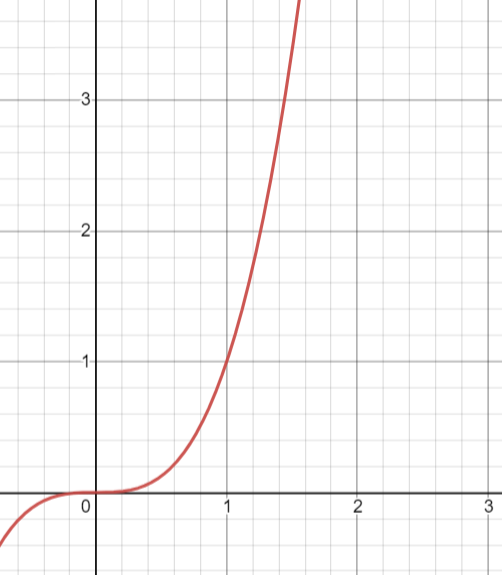
\includegraphics[scale=0.65]{Time_complex.png}
\begin{center}\textbf{Figure 1:} Time Complexity \end{center}
\subsection{Space Complexity}
2D representation of Space complexity are plotted :\newline\\
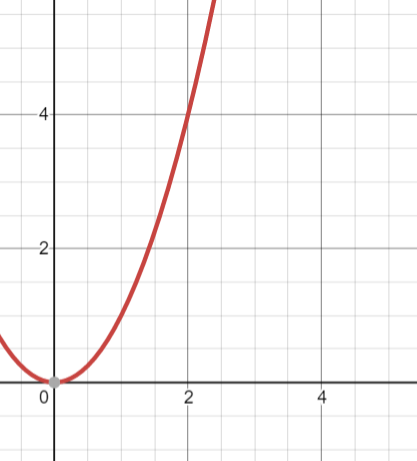
\includegraphics[scale=0.75]{Space_complex.png}
\begin{center}\textbf{Figure 2:} Space Complexity\end{center}

\section{Conclusion}
Brute force solution is to consider every possible assignment implies a complexity of Ω(n!).
The Hungarian algorithm, aka Munkres assignment algorithm, utilizes the following theorem for polynomial runtime complexity (worst case O(n$^{3}$) and guaranteed optimality

\section{Acknowledgment}
We are very much grateful to our Course instructor Mr.Rahul kala and our mentor, Mr.Md Meraz, who have provided the great opportunity to do this wonderful work on the subject of Data Structure and Algorithm Analysis .

\section{References}

We have referred [2] and [3] to clear the basic concepts of optimal assignment solution.Reference [1] helped us , to develop solution of hungarian method.
\begin{thebibliography}{00}
\bibitem{b1}https://www.geeksforgeeks.org/hungarian-algorithm-assignment-problem-set-1-introduction/
\bibitem{b2}https://www.engineeringenotes.com/project-management-2/operations-research/assignment-problem-meaning-methods-and-variations-operations-research/15652
\bibitem{b3}https://en.wikipedia.org/wiki/Hungarian_algorithm
\end{thebibliography}

\section{Appendix}

\subsection{Project link on Github:}
https://github.com/LekhanaMitta/DAA-Assignment3



\end{document}